
\documentclass[norsk,a4paper,12pt]{article}
\usepackage[T1]{fontenc} %for å bruke æøå
\usepackage[utf8]{inputenc}
\usepackage{graphicx} %for å inkludere grafikk
\usepackage{verbatim} %for å inkludere filer med tegn LaTeX ikke liker
\usepackage{mathpazo}
\usepackage{listings}
\usepackage{xcolor}
\usepackage{float}

\definecolor{background}{gray}{0.95} 
\definecolor{comment}{rgb}{0,0.5,0} 
\colorlet{keyword}{blue} 
\colorlet{string}{red} 
\lstset{numbers=left, 
	title=\lstname, 
	numberstyle=\tiny, 
	breaklines=true, 
	tabsize=4, 
	language=Python,	
	morekeywords={with,super,as},, 
	frame=single, 
	basicstyle=\footnotesize\tt, 
	commentstyle=\color{comment}, 
	keywordstyle=\color{keyword}, 
	stringstyle=\color{string}, 
	backgroundcolor=\color{background}, 
	showstringspaces=false, 
	numbers=left, 
	numbersep=5pt, 
	literate= 
		{æ}{{\ae}}1 
		{å}{{\aa}}1 
		{ø}{{\o}}1 
		{Æ}{{\AE}}1 
		{Å}{{\AA}}1 
		{Ø}{{\O}}1 
	} 
\bibliographystyle{plain}

\title{FYS 2130 Oblig3}
\author{Adnan Vrevic}
\date{\today}
\begin{document}

\maketitle


\section*{Oppgave 2}

Hvis man ikke filtrerer bort frekvenser på over halve samplingsfrekvensen vil ikke lydsignalet nødvendigvis bli entydig. Et stort problem ville være at frekvenser på over halve samplingsfrekvensen blir "folda" bakover og kan bli tolket som en del av det originale lydsignalet. Dette medfører en forvrengning av lyden.
1

\section*{Oppgave 14}

$sin(t)$ har nøyaktig 13 perioder innenfor $T=13 \cdot 2\pi = 26 \pi$. Frekvensen til $sin(t)$ er $f = \frac{1}{2\pi}\approx0.1592$. Rundt $f = 0.1592$ har grafen størst utlsag slik man ville forvente.

\begin{figure}[H]
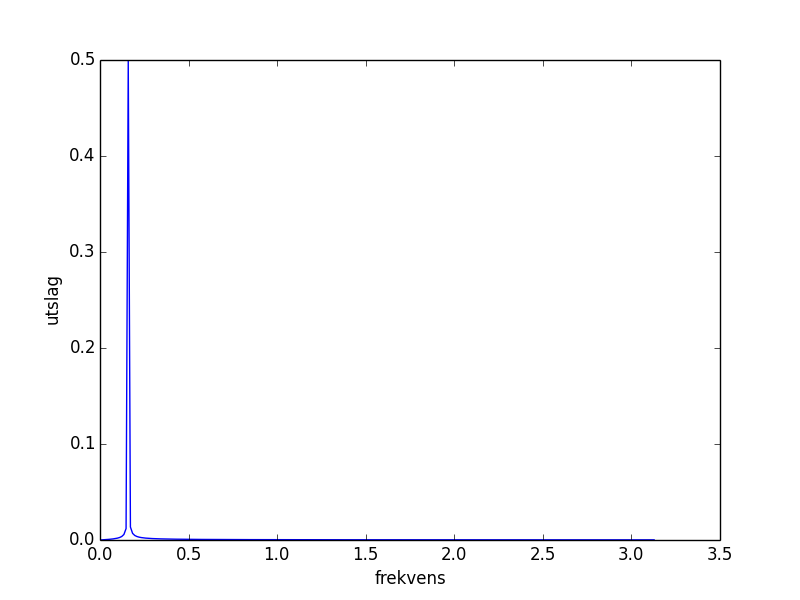
\includegraphics[width=15cm]{oppgave14.png}
\end{figure}

\section*{Oppgave 15}

Vi har fortsatt maksimalt utslag i $f =0.1592$, men det er ikke like stort som i forrige oppgave og noe spredt utover andre nærliggende frekvenser. Vi får altså ikke et like klart og entydig svar som vi får for et heltallig antall perioder for det gitte tidsintervallet.


\begin{figure}[H]
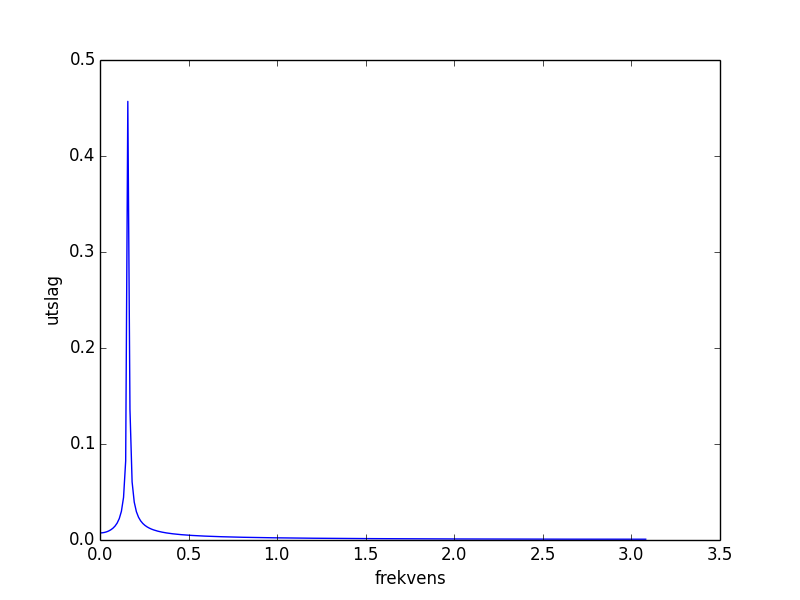
\includegraphics[width=15cm]{oppgave15.png}
\end{figure}


\section*{Oppgave 16}

vi bruker at en sum over oddetall sinusfunksjoner konvergerer mot en firkantpuls:

\begin{equation}
\Sigma_{k=0}^N \frac{1}{2k+1}sin((2k+1)t)
\end{equation}

Plottet viser maksimalt utslag for frekvensen $f=\frac{1}{2\pi} (k=0)$, deretter $f=\frac{3}{2\pi} (k=1)$ med amplitude på $\frac{1}{3}$ av den for $(k =0)$. Deretter $f=\frac{5}{2\pi} $ med amplitude på $\frac{1}{5}$ av den for $(k=0)$ osv. til vi treffer halve samplingsfrekvensen etter $f=\frac{31}{2\pi} $. Dette stemmer overens med amplitude og frekvens for de sinusfunksjonene vi superponerer.


\begin{figure}[H]
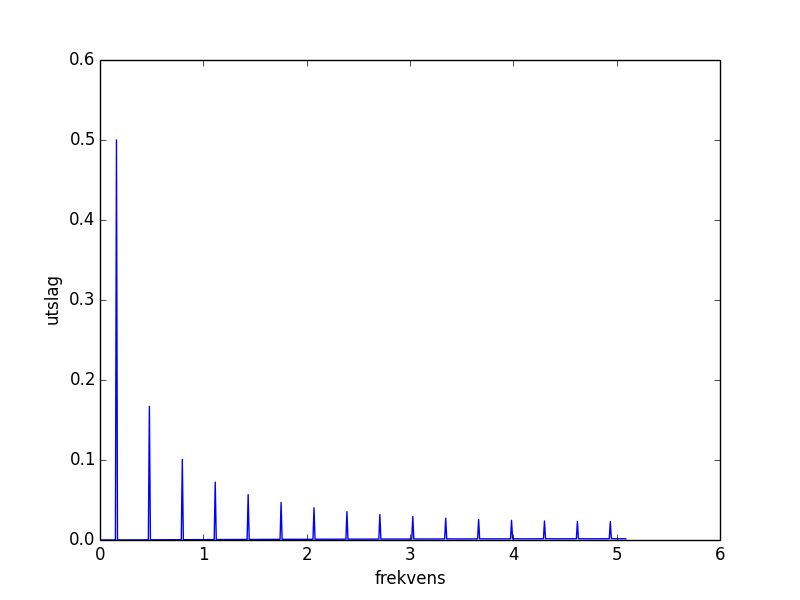
\includegraphics[width=15cm]{oppgave16.png}
\end{figure}

\section*{Oppgave 8}


\section*{Vedlegg}


\lstinputlisting{Oppgave14.py}


\lstinputlisting{oppgave15.py}

\lstinputlisting{Oppgave16.py}

\lstinputlisting{oppgave11.py}



\end{document}